\documentclass[aspectratio=169, utf8]{beamer}
\usepackage{indentfirst}
\usepackage{ctex}
\usepackage{setspace}
\usepackage{multicol}
\usepackage{cite}
\usepackage{color}
\usepackage{xcolor}
\usepackage{qrcode}
\usepackage{booktabs}
\usepackage{array}
\usepackage{colortbl}
\usepackage{tikz}
\usepackage{beamerfoils}

\setbeamertemplate{navigation symbols}{}
\usetheme{Berlin}
\usecolortheme{dolphin}
\usefonttheme{serif}
\definecolor{Fore}{RGB}{51, 51, 178}
\pgfdeclareimage[width=2.5cm]{BUPT}{./resources/logo_full.png}

\title[北京邮电大学]{北京邮电大学寒假宣讲}
\subtitle{江苏省江阴高级中学}
\author{夏锦熠、黄凯博}
\institute[网络空间安全学院]{北京邮电大学网络空间安全学院}
\date{}

\setstretch{1.2}
\setlength{\parindent}{2em}
\setlength{\parskip}{1em}

\begin{document}

\section*{封面}

\begin{frame}
    \centering
    \vspace{1em}
    
\includegraphics[width=0.18\textwidth]{./resources/logo.png}\\[0pt]
    \titlepage
\end{frame}

\setlength{\parskip}{0.5em}
\logo{\vspace*{5.8cm}\pgfuseimage{BUPT}}

\begin{frame}{目录}
    \begin{multicols}{2}
        \tableofcontents
    \end{multicols}
\end{frame}

\section{北邮历史}

\begin{frame}{目录}
    \begin{multicols}{2}
        \tableofcontents[sectionstyle=show,subsectionstyle=hide,currentsection]
    \end{multicols}
\end{frame}

\begin{frame}{厚德博学,敬业乐群}
    \begin{columns}
        \column{0.6\textwidth}
        \setlength{\parindent}{2em}

        北京邮电大学创建于 1955 年,是中华人民共和国\textcolor{Fore}{\textbf{第一所邮电高等学府}}。

        六十余载风雨砥砺,六十余载春华秋实。
        明光之北、蓟门之南,
        古老的城墙,见证了永不消逝的电波;
        鸿雁翱翔、银杏巍巍,
        坚实的土地,承载了信息黄埔的传奇。

        \column{0.4\textwidth}
        \centering
        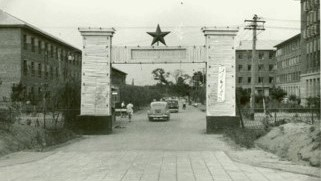
\includegraphics[width=0.8\textwidth]{./resources/1.jpg}\\%[1em]

        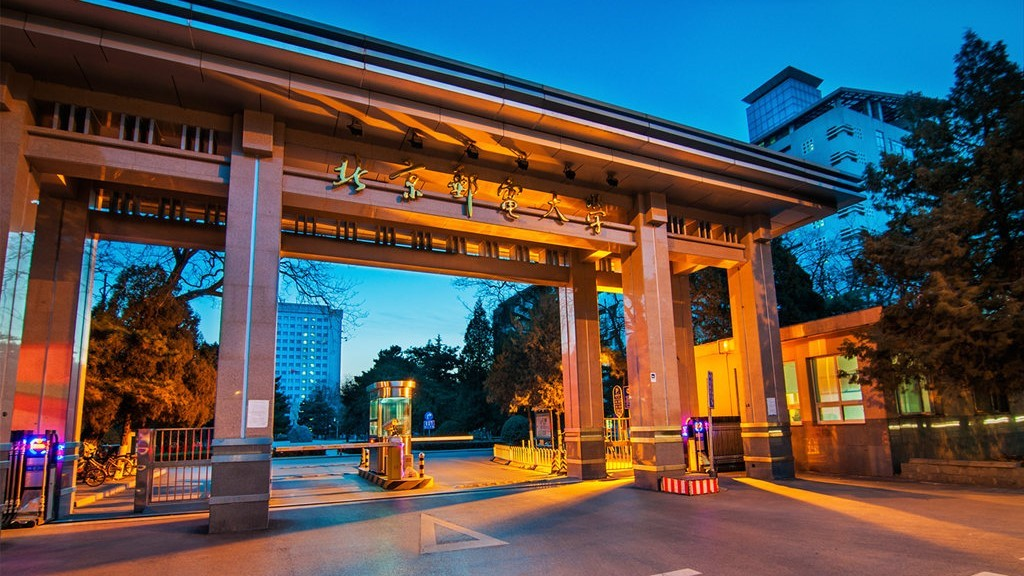
\includegraphics[width=0.8\textwidth]{./resources/2.jpg}
    \end{columns}
\end{frame}

\begin{frame}{历史中的多个第一}
    \begin{columns}
        \column{0.27\textwidth}
        \centering
        \scriptsize
        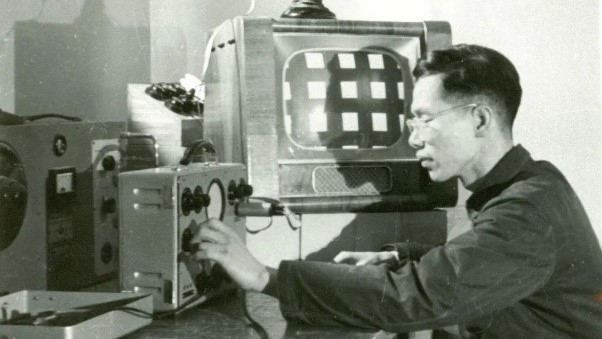
\includegraphics[width=0.9\textwidth]{./resources/3.jpg}

        我国\textcolor{Fore}{\textbf{第一座}}教学实验用黑白电视收发系统\\[1em]

        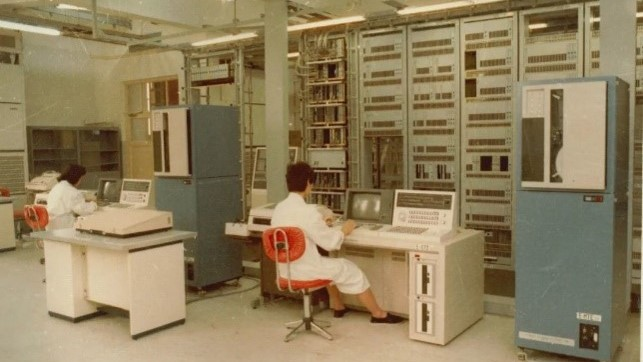
\includegraphics[width=0.9\textwidth]{./resources/4.jpg}

        我国\textcolor{Fore}{\textbf{第一台}}程控数字交换机

        \column{0.27\textwidth}
        \centering
        \scriptsize
        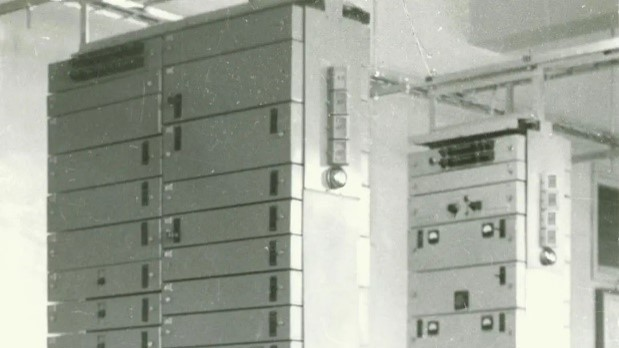
\includegraphics[width=0.9\textwidth]{./resources/5.jpg}

        我国\textcolor{Fore}{\textbf{第一台}}国产三路载波机

        \vspace{2.3em}

        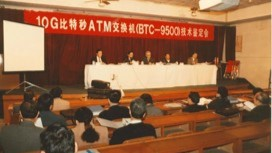
\includegraphics[width=0.9\textwidth]{./resources/6.jpg}

        我国\textcolor{Fore}{\textbf{第一台}} ATM 交换机

        \column{0.27\textwidth}
        \centering
        \scriptsize
        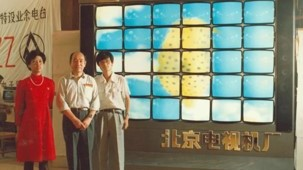
\includegraphics[width=0.9\textwidth]{./resources/7.jpg}

        我国\textcolor{Fore}{\textbf{第一台}}组合屏电视墙

        \vspace{2.3em}

        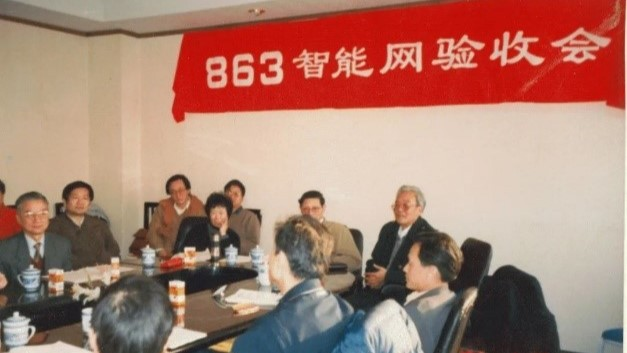
\includegraphics[width=0.9\textwidth]{./resources/8.jpg}

        我国\textcolor{Fore}{\textbf{第一个}}智能网实验网

        \column{0.19\textwidth}
        \setlength{\parindent}{2em}

        通信业从百废待兴,到探索 6G 科技前沿,北邮人见证、参与、贡献、探索,一路走来,硕果累累。

    \end{columns}
\end{frame}

\section{北邮实力}

\subsection*{学科建设}

\begin{frame}{目录}
    \begin{multicols}{2}
        \tableofcontents[sectionstyle=show,subsectionstyle=hide,currentsection]
    \end{multicols}
\end{frame}

\begin{frame}{学科突出,专业一流}
    \begin{itemize}
        \item 2017 年、2022 年北京邮电大学均入选\textcolor{Fore}{\textbf{“双一流”建设高校}}
        \item \textcolor{Fore}{\textbf{“信息与通信工程”}}和\textcolor{Fore}{\textbf{“计算机科学与技术”}}入选\textcolor{Fore}{\textbf{“双一流”建设学科}}
        \item 国内具有全通信领域研究开发能力的大学
        \item 教育部直属的\textcolor{Fore}{\textbf{首批“211工程”}}院校
        \item 国家首批硕士与博士学位授权单位
        \item 全国 56 所设立研究生院的高校之一
        \item \textcolor{Fore}{\textbf{“985优势学科创新平台”}}项目重点建设高校
    \end{itemize}
\end{frame}

\begin{frame}{学科突出,专业一流}
    \begin{columns}
        \column{0.5\textwidth}
        \begin{block}{开展“双一流”建设的两个学科群}
            \begin{multicols}{2}
                \centering

                信息网络科学与技术学科群\\

                计算机科学与网络安全学科群
            \end{multicols}
        \end{block}

        \column{0.5\textwidth}
        \setlength{\parindent}{2em}

        我校\textcolor{Fore}{\textbf{“双一流”学科建设}}涵盖了我校信通、电子、计算机、网安、人工智能等\textcolor{Fore}{\textbf{大部分}}本科教学学院,
        辐射和影响到我校\textcolor{Fore}{\textbf{绝大部分}}招生专业和招生计划。
    \end{columns}
\end{frame}

\begin{frame}{教育部第四轮学科评估}
    \begin{block}{3 个一级学科被评为 A 类}
        \centering
        \begin{columns}
            \column{0.3\textwidth}
            \begin{center}
                \Large\textcolor{Fore}{\textbf{A$^+$}}

                \normalsize 信息与通信工程\\(全国\textcolor{Fore}{\textbf{第一}})
            \end{center}

            \column{0.3\textwidth}
            \begin{center}
                \Large\textcolor{Fore}{\textbf{A}}

                \normalsize 计算机科学与技术
            \end{center}

            \column{0.3\textwidth}
            \begin{center}
                \Large\textcolor{Fore}{\textbf{A$^-$}}

                \normalsize 电子科学与技术
            \end{center}
        \end{columns}

        \vspace{1em}
    \end{block}

    \scriptsize\vspace{1em}

    \begin{columns}
        \column{0.4\textwidth}
        \centering
        \Large\textcolor{Fore}{\textbf{5 个}}

        \normalsize 一级学科被评为 \textcolor{Fore}{\textbf{B 类}}

        \column{0.4\textwidth}
        \centering
        \Large\textcolor{Fore}{\textbf{3 个}}

        \normalsize 一级学科被评为 \textcolor{Fore}{\textbf{C 类}}

    \end{columns}
\end{frame}

\begin{frame}{学科突出,专业一流}
    \begin{multicols}{2}
        \begin{center}
            \LARGE\textcolor{Fore}{\textbf{21 个}}\\[0.5em]

            \normalsize 国家级\\一流本科专业\\建设点
        \end{center}

        \begin{center}
            \LARGE\textcolor{Fore}{\textbf{16 个}}\\[0.5em]

            \normalsize 省级\\一流本科专业\\建设点
        \end{center}
    \end{multicols}

    国家级和省级一流本科专业建设点覆盖全校\textcolor{Fore}{\textbf{接近 95\%}} 的本科学生。
\end{frame}

\begin{frame}{学科突出,专业一流}
    \begin{itemize}
        \item \textcolor{Fore}{\textbf{计算机科学}}进入 \textcolor{Fore}{\textbf{ESI 前千分之一}}。
        \item 信息材料科学与工程、网络空间治理入选\textcolor{Fore}{\textbf{北京高校“高精尖”学科}}。
        \item 2021 年,计算机科学拔尖学生培养基地成功入选\textcolor{Fore}{\textbf{教育部基础学科拔尖学生培养计划 2.0 基地}}。
    \end{itemize}

    学科涵盖了理、工、文、法、经济、管理、艺术等 7 个学科门类,初步形成了\textcolor{Fore}{\textbf{信息学科优势突出}}、\textcolor{Fore}{\textbf{工管文理相互支撑}}的多科性学科架构。
\end{frame}

\subsection*{师资科研}

\begin{frame}{师资强大,名家荟萃}
    \begin{multicols}{2}
        \begin{itemize}
            \item 院士:\textcolor{Fore}{\textbf{13 人}}
            \item 专任教师:\textcolor{Fore}{\textbf{1715 人}}
            \item 正、副高级职称教师:\textcolor{Fore}{\textbf{1009 人}}
            \item 外籍教师:\textcolor{Fore}{\textbf{100$^+$ 人}}
            \item 国家级教学名师:\textcolor{Fore}{\textbf{2 人}}
            \item 国家杰出青年科学基金获得者:\textcolor{Fore}{\textbf{16 人}}
            \item 国家高层次人才特殊支持计划领军人才:\textcolor{Fore}{\textbf{11 人}}
            \item 国家优秀青年科学基金获得者:\textcolor{Fore}{\textbf{14 人}}
            \item 国家自然科学基金委员会创新研究群体学术带头人:\textcolor{Fore}{\textbf{5 人}}
            \item 青年拔尖人才:\textcolor{Fore}{\textbf{8 人}}
            \item 享受政府特殊津贴专家:\textcolor{Fore}{\textbf{100$^+$ 人}}
            \item “新世纪百千万人才工程”国家级人选:\textcolor{Fore}{\textbf{9 人}}
        \end{itemize}
    \end{multicols}
\end{frame}

\begin{frame}{科研突出,实力显著}
    \begin{columns}
        \column{0.5\textwidth}
        \setlength{\parindent}{2em}

        学校科研坚持瞄准世界信息通信科技前沿、聚焦\textcolor{Fore}{\textbf{“网络强国”}}国家重大战略需求、服务\textcolor{Fore}{\textbf{“数字经济”}}高质量发展、面向人民生命健康,
        加强“从 0 到 1 ”基础研究、应用基础研究,突出关键共性技术、前沿引领技术、现代工程技术、颠覆性技术和交叉领域创新,
        承担大量国家级和省部级科技计划项目。

        \column{0.5\textwidth}
        \begin{itemize}
            \item 国家重点实验室:\textcolor{Fore}{\textbf{2 个}}
            \item 国家工程研究中心:\textcolor{Fore}{\textbf{2 个}}
            \item 国家级国际科技合作基地:\textcolor{Fore}{\textbf{1 个}}
            \item 教育部重点实验室:\textcolor{Fore}{\textbf{4 个}}
            \item 教育部工程研究中心:\textcolor{Fore}{\textbf{2 个}}
            \item 网络空间国际治理研究基地:\textcolor{Fore}{\textbf{1 个}}
            \item 北京实验室:\textcolor{Fore}{\textbf{1 个}}
            \item 其他各类省部级科研基地:\textcolor{Fore}{\textbf{26 个}}
        \end{itemize}
    \end{columns}
\end{frame}

\begin{frame}{科研突出,实力显著}
    \begin{columns}
        \column{0.6\textwidth}
        \setlength{\parindent}{2em}

        学校充分发挥学科、科技、人才优势,服务网络强国战略能力进一步提升,
        在\textcolor{Fore}{\textbf{无线通信}}、\textcolor{Fore}{\textbf{光通信}}、\textcolor{Fore}{\textbf{无线网络定位}}、
        \textcolor{Fore}{\textbf{未来网络}}、\textcolor{Fore}{\textbf{文化大数据}}等领域实现基础研究和关键核心技术突破以及标准体系制定,达到一流水平。
        在\textcolor{Fore}{\textbf{国家空间站建设}}和\textcolor{Fore}{\textbf{科技冬奥}}、\textcolor{Fore}{\textbf{科技扶贫}}、\textcolor{Fore}{\textbf{科技抗疫}}等国家重大科研需求中贡献了北邮科技力量。

        \column{0.4\textwidth}
        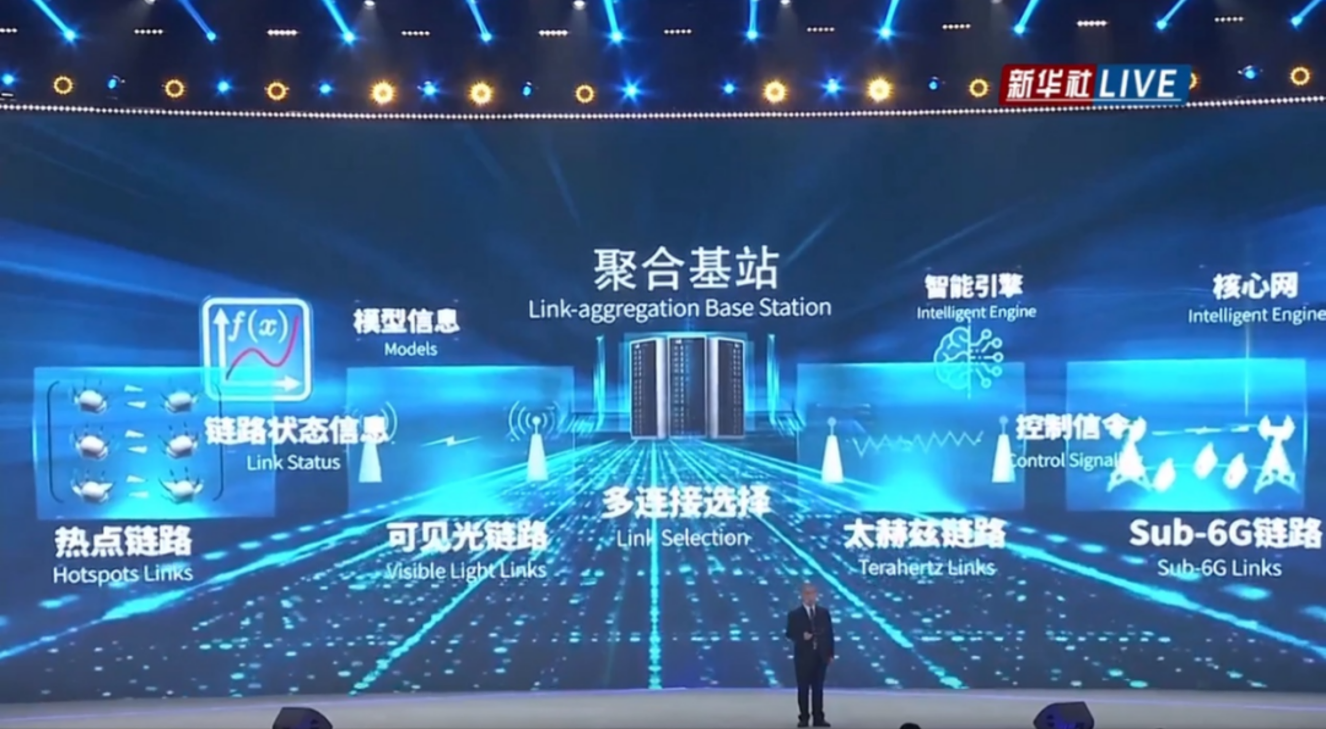
\includegraphics[width=\textwidth]{./resources/9.png}
        \setlength{\parindent}{2em}
        \scriptsize

        在 2022 世界互联网大会上,北邮网安院陶小峰教授发布成果《EAGLE 6G:面向 6G 无线高速接入原型系统及测试环境》。
    \end{columns}
\end{frame}

\subsection*{人才培养}

\begin{frame}{拔尖创新人才培养:叶培大创新创业学院}
    \begin{itemize}
        \item 面向全校一年级本科生在大一期末选拔优秀学生组建,每年选拔 \textcolor{Fore}{\textbf{100 人左右}},以创新创业辅修专业为培养模式,采用\textcolor{Fore}{\textbf{导师制}}、\textcolor{Fore}{\textbf{个性化}}、\textcolor{Fore}{\textbf{跨学科}}、\textcolor{Fore}{\textbf{全球化}}等特色培养。
        \item 聚焦创新创业教育与新工科融合人才培养领域,致力于培养一流创新力、领导力和国际化复合型领军人才。
        \item 围绕\textcolor{Fore}{\textbf{智能机器人}}、\textcolor{Fore}{\textbf{智慧生活}}、\textcolor{Fore}{\textbf{智慧交通}}、\textcolor{Fore}{\textbf{宽带通信与光电科技}}四个研究方向。
        \item 不定期组织学生参与国际名校短期项目,学习前沿科技、巩固英语交流能力、拓宽国际视野。
        \item 提供专属学习环境,进入前沿技术主题实验室,设立专项基金,注重提升学生综合应用能力。
    \end{itemize}
\end{frame}

\begin{frame}{拔尖创新人才培养:叶培大创新创业学院}
    截至目前,实验班共获得国家级学科竞赛、双创竞赛各类奖项\textcolor{Fore}{\textbf{共 122 项}},其中\textcolor{Fore}{\textbf{国家级竞赛一等奖 41 项}};
    获得省市级奖项 \textcolor{Fore}{\textbf{102 项}},其中\textcolor{Fore}{\textbf{一等奖 30 项}};
    发表或被录用\textcolor{Fore}{\textbf{高水平学术论文 25 篇}},其中 \textcolor{Fore}{\textbf{SCI 检索 11 篇}}、\textcolor{Fore}{\textbf{EI 检索 14 篇}};
    申请\textcolor{Fore}{\textbf{发明专利 4 项}},获得\textcolor{Fore}{\textbf{实用新型专利 1 项}}。
    \textcolor{Fore}{\textbf{184 名}}学生被评选为 2021 届北京市优秀本科毕业生。
\end{frame}

\begin{frame}{拔尖创新人才培养:信息与通信工程学科“英才班”}
    为了贯彻国家中长期教育改革和发展规划纲要精神,信息与通信工程学院在通信工程专业成立“英才班”,
    实施本硕博贯通式培养计划,为学生配备博导作为指导教师,设立创新基金支持优秀学生更好地发挥潜能,鼓励学生参与国家重大项目研究。
    \textcolor{Fore}{\textbf{首批“英才班”实际保研比例超过 50\%。}}

    该英才班在大一下学期面向信通院学生(包括原信通院和转专业至信通院)组建。
    组建时对于报名学生学业排名有一定要求并且学院要组织专家选拔。
    往年一般 \textcolor{Fore}{\textbf{70 人左右}},安排\textcolor{Fore}{\textbf{两个班}}。
\end{frame}

\begin{frame}{拔尖创新人才培养:网络空间安全实验班}
    为培养有坚实理论基础和卓越实战技能的网安人才,网安学院面向学院内优秀学生组建实验班,通过探索性、创新性和实战性的培养机制,
    以及\textcolor{Fore}{\textbf{“以赛促学,以练促学”}}的教学模式,提高学生理论与实践能力。
    目前实验班学生已在国内外大赛中屡获佳绩。

    该实验班一般在大二上学期组建,面向网络空间安全学院内学生。组建时对于报名学生学科排名有一定要求并且学院要组织选拔。
    该实验班人数一般 \textcolor{Fore}{\textbf{30 人左右}},为一个班。
\end{frame}

\begin{frame}{学科专业类竞赛成绩优异}
    2021 年,北邮学子在各级各类学科竞赛中捷报频传,为学校赢得了广泛赞誉。
    共计有 \textcolor{Fore}{\textbf{2480 人次}}获得省部级以上各类竞赛奖励。
    其中,\textcolor{Fore}{\textbf{1540 人次}}在国家级以及国际竞赛中获奖,\textcolor{Fore}{\textbf{940 人次}}在省级竞赛中获奖。\\[1em]

    \begin{columns}
        \column{0.365\textwidth}
        \scriptsize
        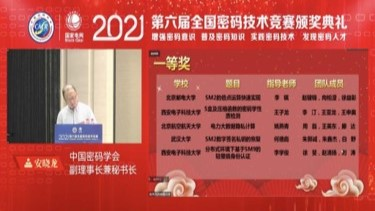
\includegraphics[width=\textwidth]{./resources/12.jpg}\\[0em]

        北邮在第六届全国密码技术竞赛中荣获一项一等奖、三项二等奖和两项三等奖。

        \column{0.365\textwidth}
        \scriptsize
        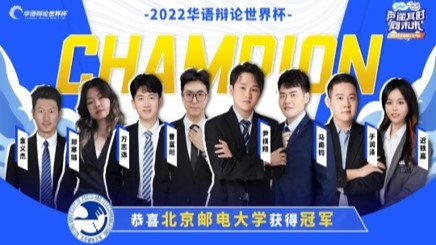
\includegraphics[width=\textwidth]{./resources/13.jpg}\\[0em]

        北邮辩论队荣获 2022 华语辩论世界杯总冠军。
    \end{columns}
\end{frame}

\section{国际学院}

\begin{frame}{目录}
    \begin{multicols}{2}
        \tableofcontents[currentsection]
    \end{multicols}
\end{frame}

\begin{frame}{国际学院(北京邮电大学玛丽女王学院)}
    \begin{columns}
        \column{0.7\textwidth}
        \small
        \setlength{\parindent}{2em}

        北京邮电大学国际学院于 2004 年成立,是北京邮电大学校内实施中外合作办学项目的学院,至今已有 \textcolor{Fore}{\textbf{18 年}}办学经验。
        国际学院立足本土,面向全球,深度融合中英两校优质教育资源,服务国家\textcolor{Fore}{\textbf{“网络强国”}}战略,
        面向\textcolor{Fore}{\textbf{“互联网+”}}和\textcolor{Fore}{\textbf{“AI+”}}新经济发展需求,
        坚持“厚基础、宽口径、促交叉、强实践”的培养理念,实施跨学科融合创新的 ICT (Information and Communication Technology) 国际化人才培养模式,
        培养具有爱国情怀、国际视野、术业精良、能力突出、适应全球化竞争环境的高素质创新人才和行业领军人才。

        \column{0.3\textwidth}
        \centering
        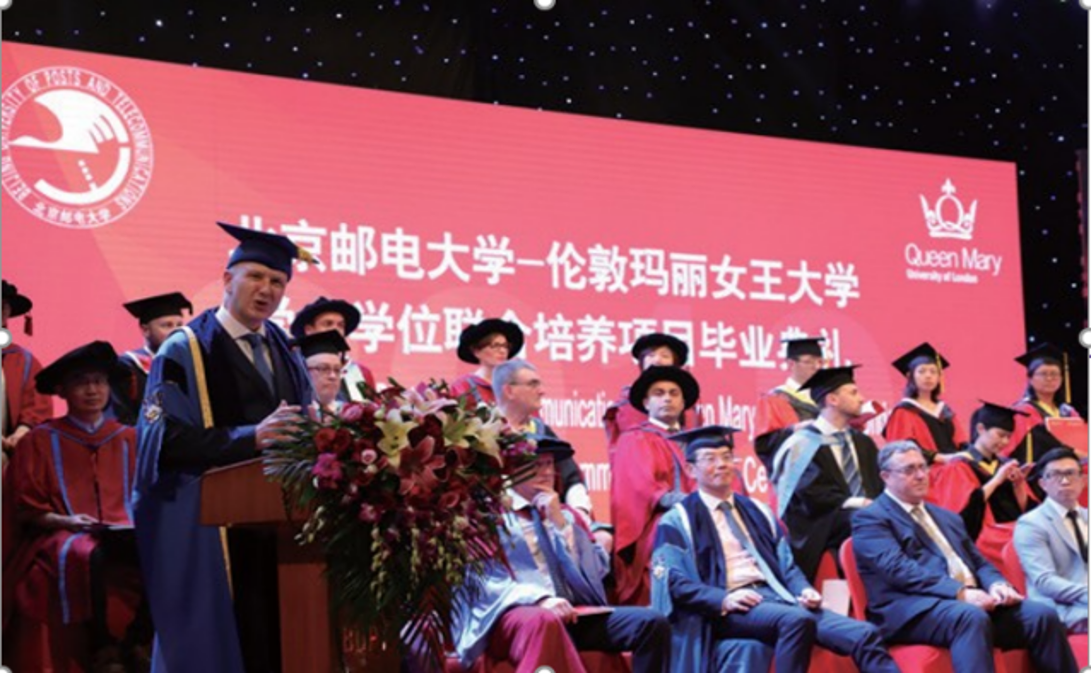
\includegraphics[width=\textwidth]{./resources/10.png}
        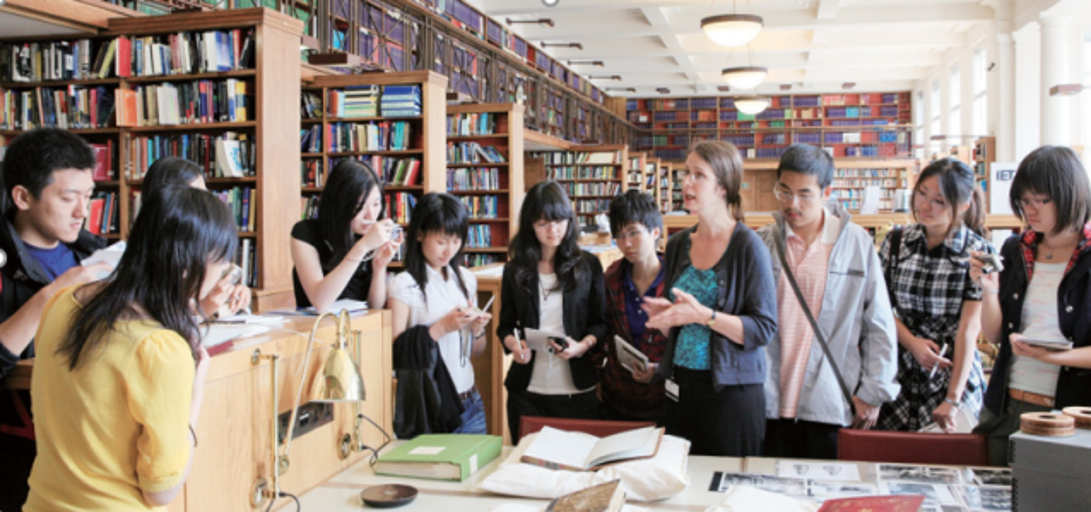
\includegraphics[width=\textwidth]{./resources/11.png}
    \end{columns}
\end{frame}

\begin{frame}{合作院校:英国伦敦玛丽女王大学}
    \begin{columns}
        \column{0.5\textwidth}
        \setlength{\parindent}{2em}

        英国伦敦玛丽女王大学是位于英国伦敦的著名综合研究型公立大学,其历史可追溯至 1785 年,现已有\textcolor{Fore}{\textbf{两百余年}}历史,
        是包括牛津、剑桥等英国顶级高校在内的\textcolor{Fore}{\textbf{罗素 (Russel) 大学集团}}成员之一、
        \textcolor{Fore}{\textbf{英国科学与工程联盟}}成员、\textcolor{Fore}{\textbf{艾伦图灵研究院建设高校}}之一。

        \column{0.5\textwidth}
        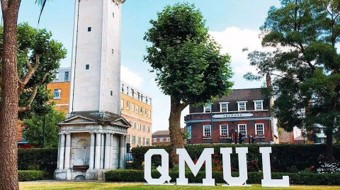
\includegraphics[width=\textwidth]{./resources/14.jpg}
    \end{columns}
\end{frame}

\begin{frame}{合作院校:英国伦敦玛丽女王大学}
    \begin{itemize}
        \item 2022年QS世界大学排名\textcolor{Fore}{\textbf{第 117 位}}
        \item 英国2021卓越研究框架 (REF) 中,科研质量与科研成果名列全英\textcolor{Fore}{\textbf{第 7}}
        \item 十余个学科在 REF 2021 中排名全英\textcolor{Fore}{\textbf{前 10}}
        \item 计算机科学和信息学科研影响力位列全英\textcolor{Fore}{\textbf{第 1}}
        \item 工程学科研质量与科研成果位列全英\textcolor{Fore}{\textbf{第 2}}
        \item 该校已培养出 \textcolor{Fore}{\textbf{9 位诺贝尔奖获得者}}和 \textcolor{Fore}{\textbf{55 位院士}}
        \item 全英\textcolor{Fore}{\textbf{第一所}}荣获 NCCPE Platinum-level Engage Watermark 铂金认证的大学
    \end{itemize}
\end{frame}

\begin{frame}{国际学院(北京邮电大学玛丽女王学院)}
    \begin{columns}
        \column{0.25\textwidth}
        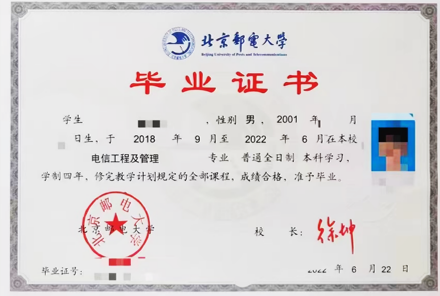
\includegraphics[width=\textwidth]{./resources/15.png}\\
        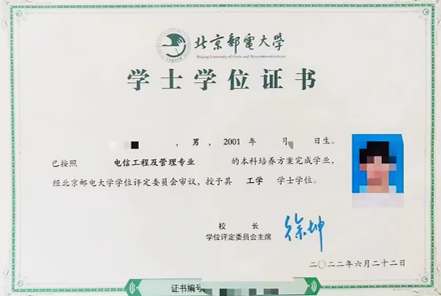
\includegraphics[width=\textwidth]{./resources/16.png}

        \column{0.25\textwidth}
        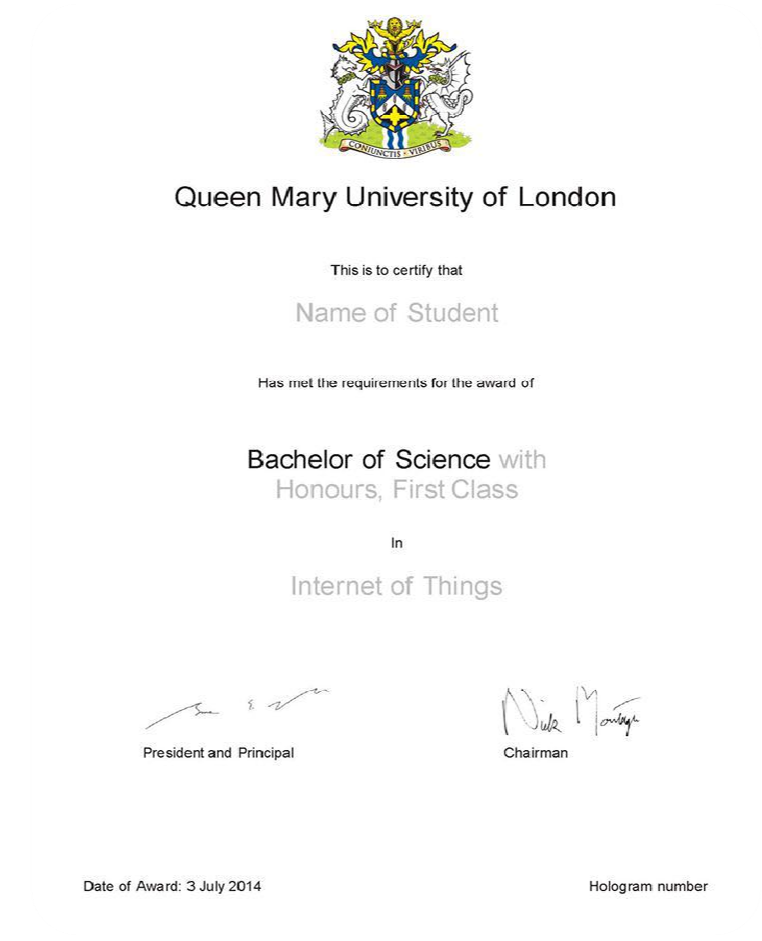
\includegraphics[width=\textwidth]{./resources/17.png}

        \column{0.5\textwidth}
        \footnotesize
        \begin{itemize}
            \item \textcolor{Fore}{\textbf{2022 级教学安排}}

                  四年均在国内完成。第一年双语授课,第二年起全英语授课。我校与英方大学各承担 50\% 的课程。

            \item \textcolor{Fore}{\textbf{江苏招生方式}}

                  以\textcolor{Fore}{\textbf{“北京邮电大学(宏福校区)”}}的名称\textcolor{Fore}{\textbf{单设专业组}}在本科一批招生。

            \item \textcolor{Fore}{\textbf{毕业去向}}

                  毕业生获得\textcolor{Fore}{\textbf{英国一等学位}}比例高达 \textcolor{Fore}{\textbf{39.4\%}},
                  \textcolor{Fore}{\textbf{出国深造率约 64\%}},有\textcolor{Fore}{\textbf{超过 50\%}} 的毕业生被\textcolor{Fore}{\textbf{全球百强高校}}录取,
                  \textcolor{Fore}{\textbf{读研率约 80\%}}。
        \end{itemize}
    \end{columns}
\end{frame}

\section{就业深造}

\begin{frame}{目录}
    \begin{multicols}{2}
        \tableofcontents[currentsection]
    \end{multicols}
\end{frame}

\subsection*{毕业深造}

\begin{frame}{本科毕业深造}
    \begin{columns}
        \column{0.3\textwidth}
        \centering
        \LARGE\textcolor{Fore}{\textbf{61.34\%}}\\[0.5em]

        \normalsize 毕业生深造率

        \column{0.3\textwidth}
        \centering
        \LARGE\textcolor{Fore}{\textbf{49.35\%}}\\[0.5em]

        \normalsize 境内读研率

        \column{0.3\textwidth}
        \centering
        \LARGE\textcolor{Fore}{\textbf{11.99\%}}\\[0.5em]

        \normalsize 境外读研率
    \end{columns}

    \normalsize
    \vspace{1em}

    2022 年学校本科毕业生境内升学人数共计 1815 人,境内升学率为 49.35\%。
    其中,\textcolor{Fore}{\textbf{超过 80\% 留在本校读研}}。
    除本校外,录取人数排名前三的学校依次为\textcolor{Fore}{\textbf{中国科学院大学}}、\textcolor{Fore}{\textbf{清华大学}}和\textcolor{Fore}{\textbf{北京大学}}。
\end{frame}

\begin{frame}{本科毕业深造}
    \begin{columns}
        \column{0.55\textwidth}
        \setlength{\parindent}{2em}

        2022届本科生毕业生出国(境)留学 441 人,出国(境)\textcolor{Fore}{\textbf{留学率为 11.99\%}}。
        出国(境)留学毕业生主要流向\textcolor{Fore}{\textbf{英国}}(44.90\%),
        其次是\textcolor{Fore}{\textbf{中国(香港)}}(17.23\%)和\textcolor{Fore}{\textbf{新加坡}}(9.30\%)。

        就读高校包帝国理工学院、伦敦大学学院、爱丁堡大学、墨尔本大学、悉尼大学、香港大学、香港中文大学等\textcolor{Fore}{\textbf{世界百强大学}}。

        \column{0.5\textwidth}
        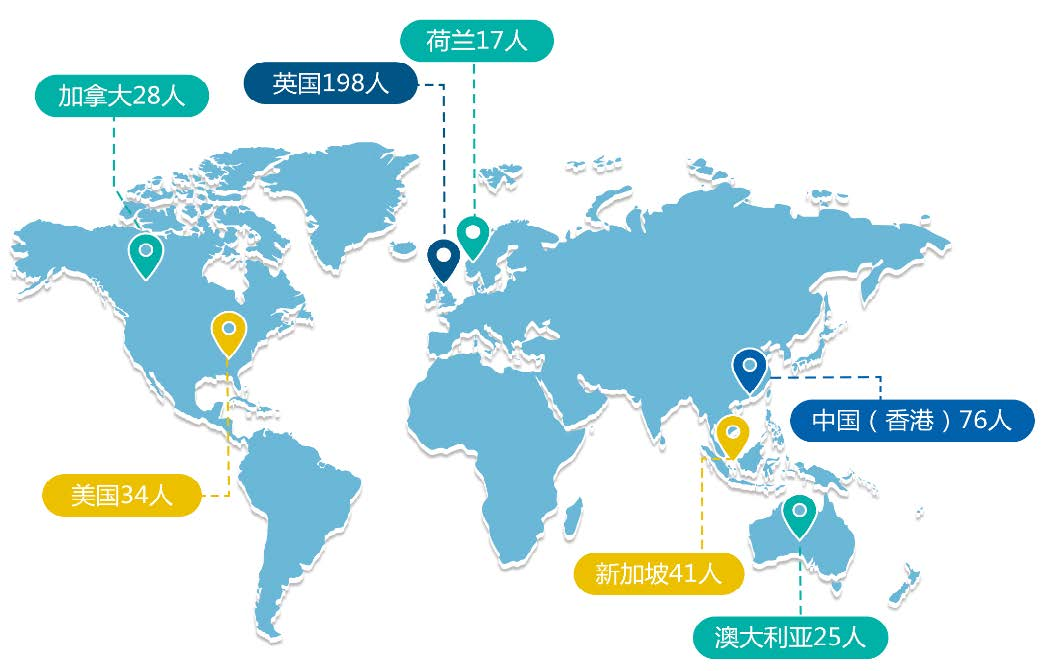
\includegraphics[width=\textwidth]{./resources/18.jpg}
    \end{columns}
\end{frame}

\subsection*{就业去向}

\begin{frame}{本科就业去向}
    \begin{columns}
        \column{0.5\textwidth}
        \setlength{\parindent}{2em}

        2022届本科生毕业主要流向单位覆盖了\textcolor{Fore}{\textbf{通信}}、\textcolor{Fore}{\textbf{互联网}}、
        \textcolor{Fore}{\textbf{信息科技}}、\textcolor{Fore}{\textbf{金融}}、\textcolor{Fore}{\textbf{航天军工}}等重点领域。
        同时,北京邮电大学毕业生紧紧围绕国家战略发展需要,以“传邮万里,国脉所系”的情怀,
        积极踊跃地选择在“一带一路”沿线地区就业,服务国家京津冀一体化建设,进入高新技术领域就业创业。

        \column{0.5\textwidth}
        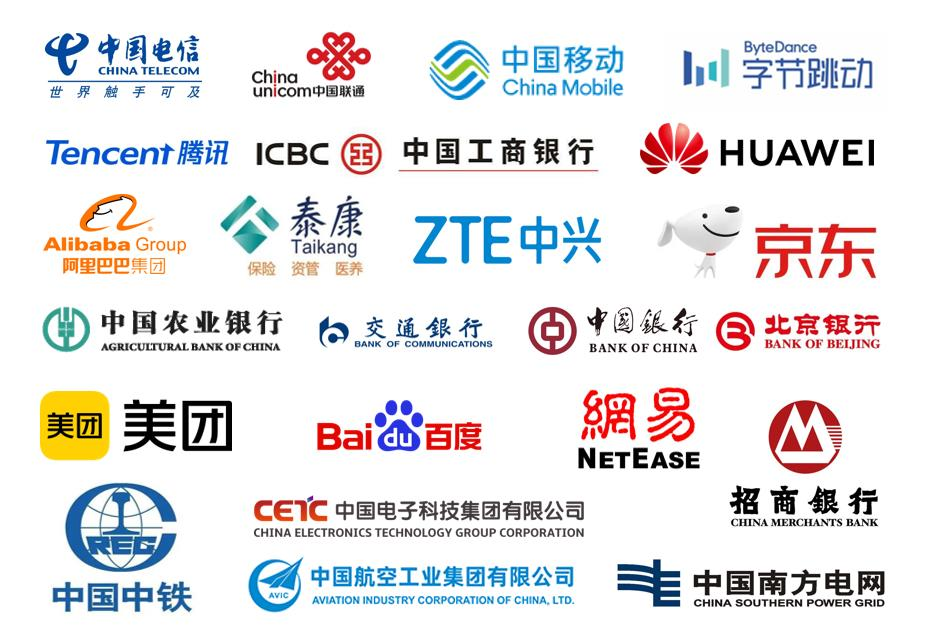
\includegraphics[width=\textwidth]{./resources/19.jpg}
    \end{columns}
\end{frame}

\section{校园生活}

\begin{frame}{目录}
    \begin{multicols}{2}
        \tableofcontents[currentsection]
    \end{multicols}
\end{frame}

\subsection*{北邮校园}

\begin{frame}{沙河校区}
    \centering
    \includegraphics[width=0.8\textwidth]{./resources/20.png}
\end{frame}

\begin{frame}{沙河校区}
    \centering
    \includegraphics[width=0.8\textwidth]{./resources/21.png}
\end{frame}

\begin{frame}{缤纷美食}
    \centering
    \includegraphics[width=0.8\textwidth]{./resources/22.png}
\end{frame}

\begin{frame}{缤纷美食}
    \centering
    \includegraphics[width=0.8\textwidth]{./resources/23.png}
\end{frame}

\begin{frame}{全中国网速最快的学校}
    \begin{columns}
        \column{0.4\textwidth}
        \setlength{\parindent}{2em}

        北京邮电大学校园网\textcolor{Fore}{\textbf{带宽不限量}},\textcolor{Fore}{\textbf{校园全覆盖}},师生\textcolor{Fore}{\textbf{全时段免费}}畅游。
        据我们所知,北邮是目前北京少有的上网全免费、不限量的高校之一。

        \column{0.3\textwidth}
        \centering
        \textcolor{Fore}{\textbf{出口带宽}}

        \Huge \textcolor{Fore}{\textbf{40}}

        \Large \textcolor{Fore}{\textbf{Gbps}}\\[1em]

        \normalsize \textcolor{Fore}{\textbf{全免费\\不限流量}}
    \end{columns}
\end{frame}

\begin{frame}{住宿条件}
    \begin{columns}
        \column{0.5\textwidth}
        \setlength{\parindent}{2em}

        沙河校区宿舍采用标准\textcolor{Fore}{\textbf{四人间}},宽敞明亮。\textcolor{Fore}{\textbf{上床下桌}}配置,方便同学们生活和学习。
        每间宿舍\textcolor{Fore}{\textbf{均安装空调暖气}},具有\textcolor{Fore}{\textbf{独立卫生间}},配备高端的家具和人性化的设计构造。
        各宿舍楼内配备\textcolor{Fore}{\textbf{开水间}}、\textcolor{Fore}{\textbf{学生活动室}}、\textcolor{Fore}{\textbf{自习室}}等,
        为学生的学习和生活提供了无限便利。住宿条件在北京高校中非常优越。

        \column{0.5\textwidth}
        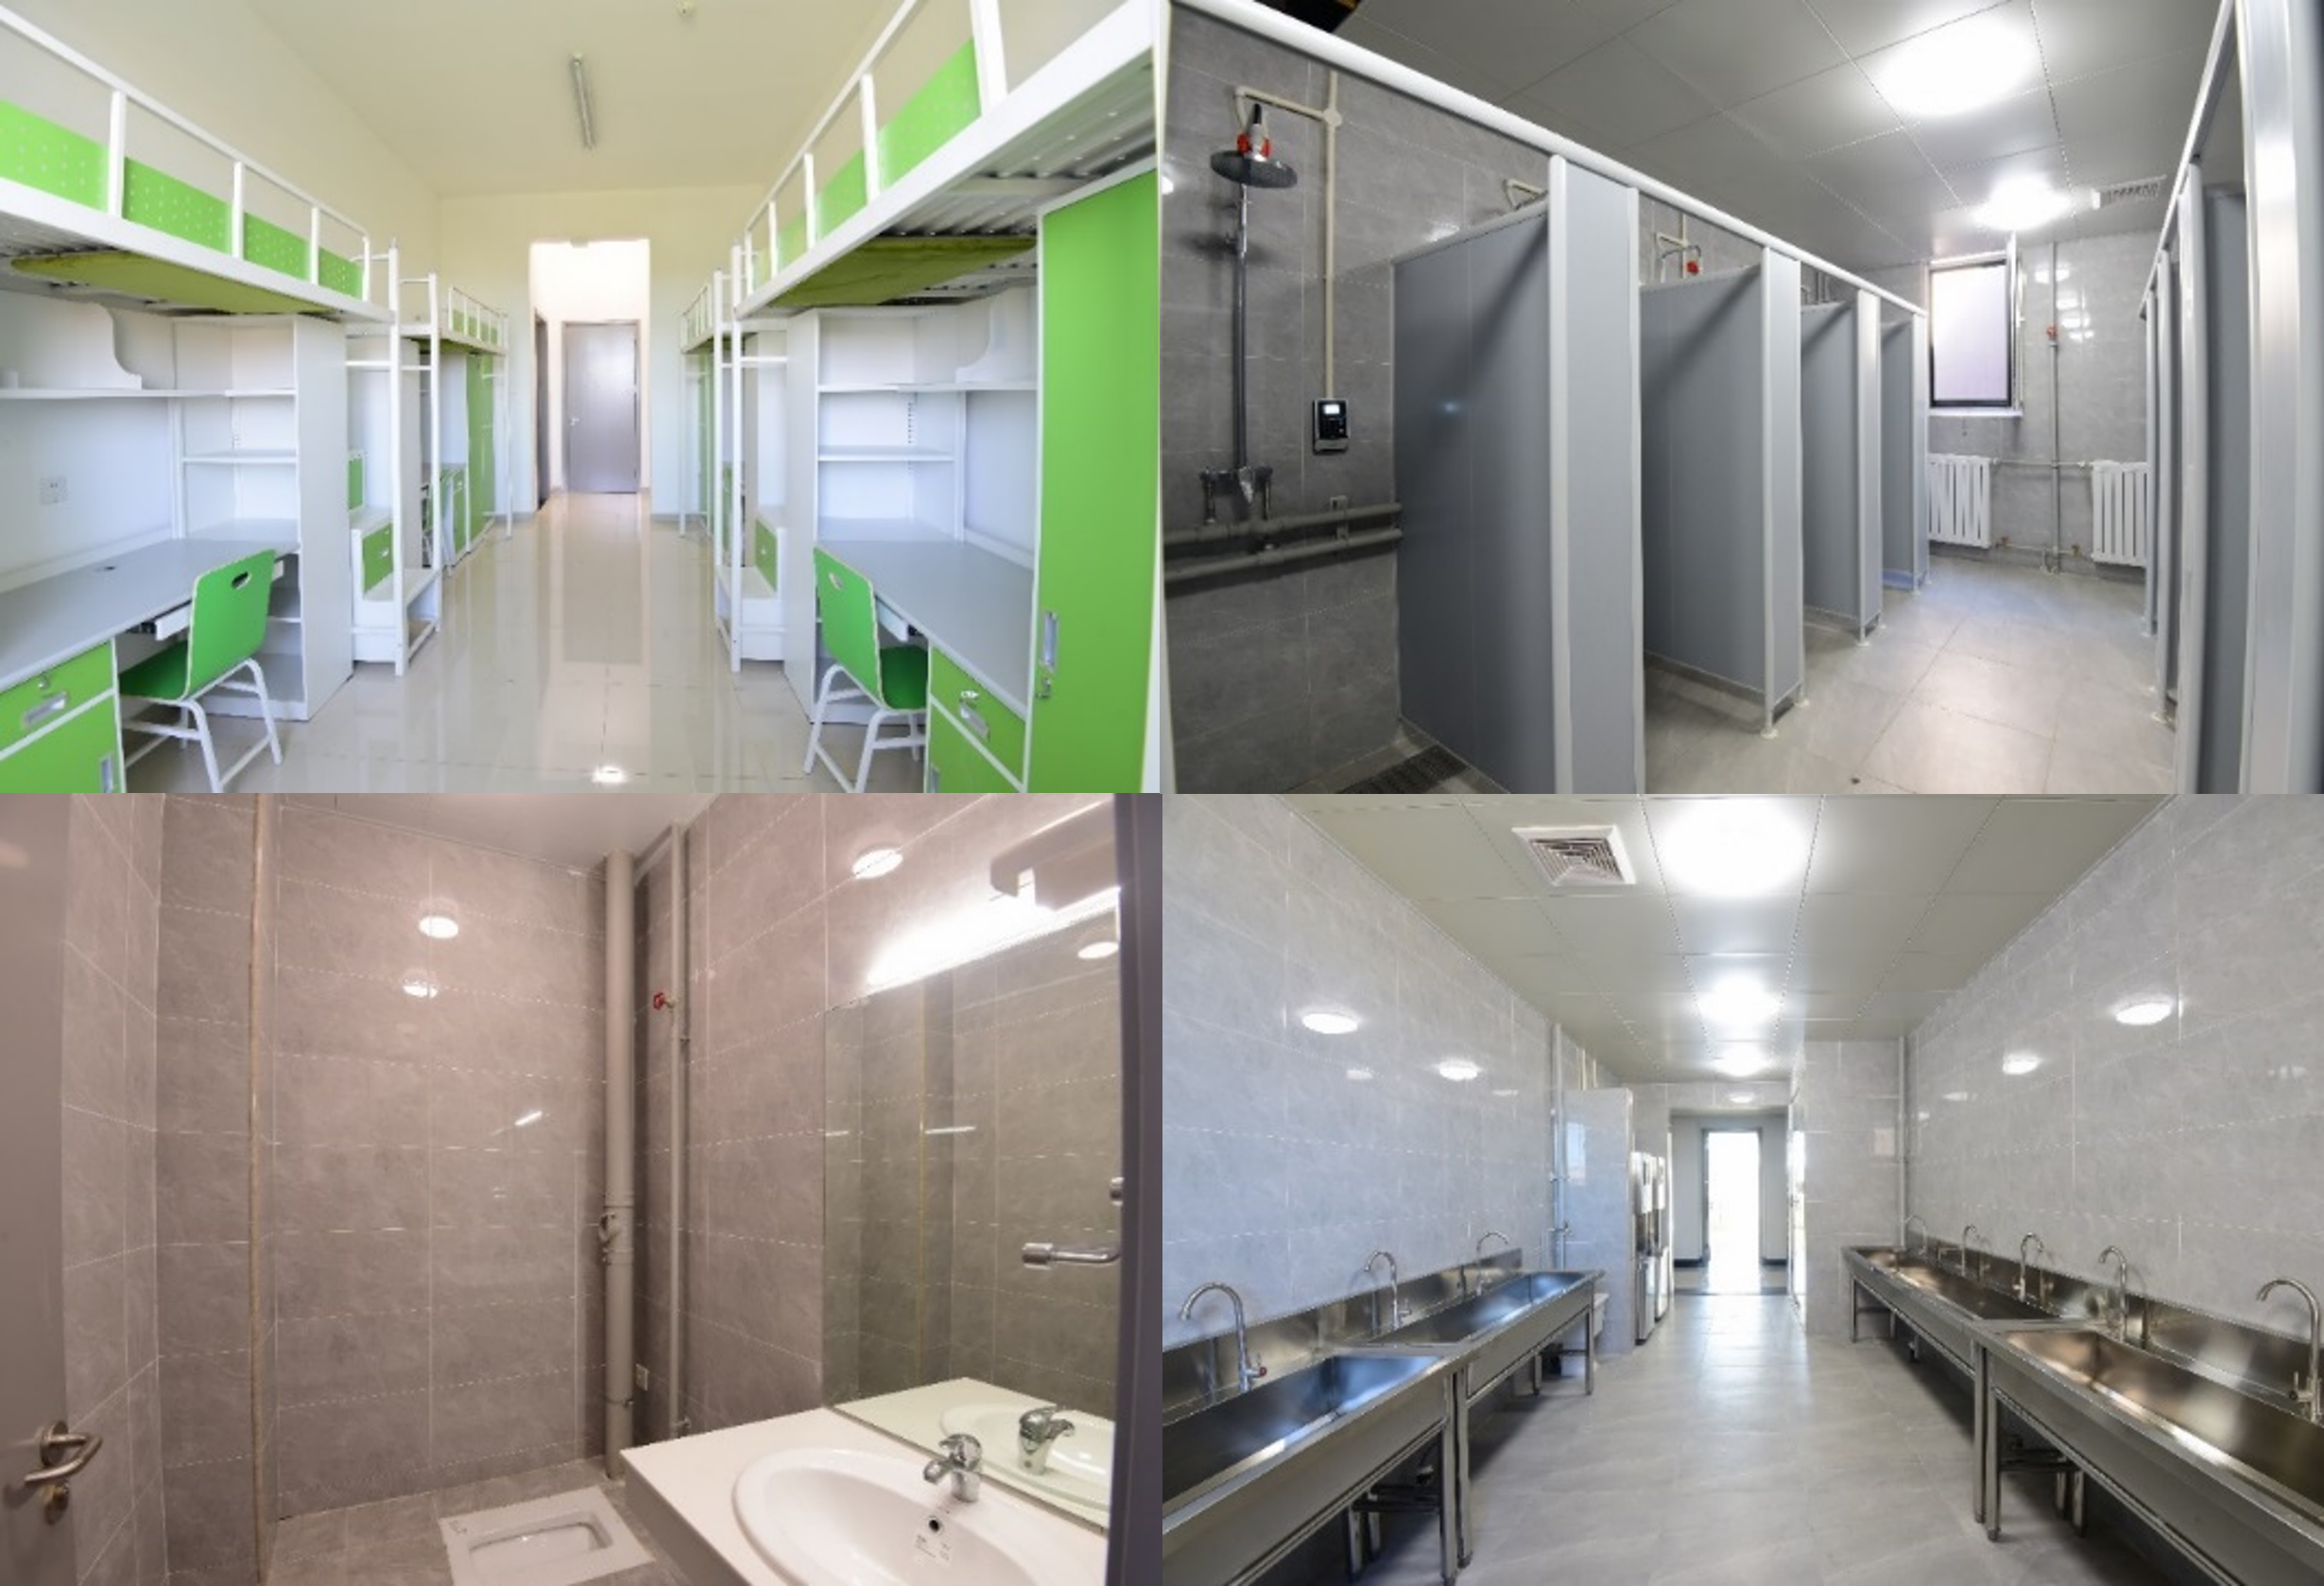
\includegraphics[width=\textwidth]{./resources/24.png}
    \end{columns}
\end{frame}

\subsection*{多彩活动}

\begin{frame}{学生社团}
    学校成立涉及学术、艺术、体育、音乐、美术、影视等多个领域的\textcolor{Fore}{\textbf{社团 90 余个}},充分建设多元校园文化,满足青年成长个性化需求。
    定期举办社团展示月、“百花节”主题晚会、社团嘉年华、游园会、“百团大战”等精品活动,丰富同学们的课余生活。\\[1em]

    \begin{columns}
        \column{0.4\textwidth}
        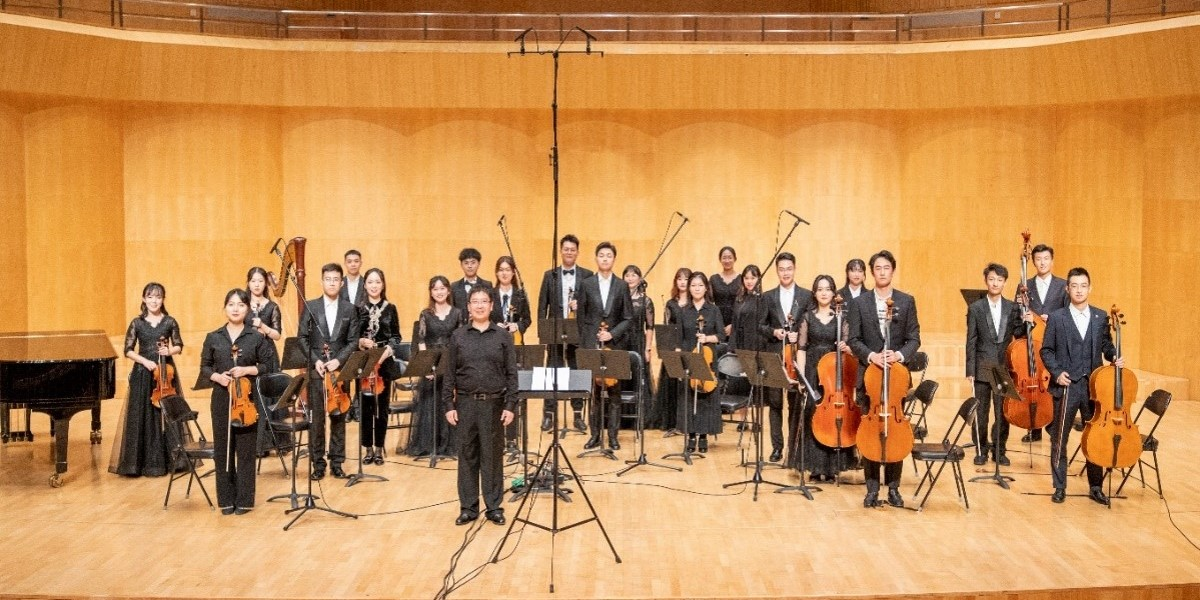
\includegraphics[width=\textwidth]{./resources/25.jpg}

        \column{0.4\textwidth}
        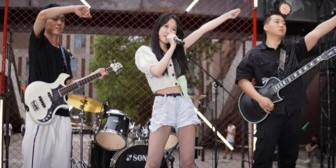
\includegraphics[width=\textwidth]{./resources/26.jpg}
    \end{columns}
\end{frame}

\begin{frame}{国庆大会}
    \begin{columns}
        \column{0.5\textwidth}
        \setlength{\parindent}{2em}

        在\textcolor{Fore}{\textbf{中华人民共和国成立 70 周年庆祝大会、阅兵式、群众游行和首都国庆联欢活动}}中,
        我校 2214 名师生、82 名港澳台群众代表组成\textcolor{Fore}{\textbf{群众游行第 13 方阵}},82 名师生参与\textcolor{Fore}{\textbf{广场合唱团演出}},
        184 名志愿者担任庆祝大会和联欢大会的\textcolor{Fore}{\textbf{志愿服务工作者}},
        102 名师生参加 9 月 29 日\textcolor{Fore}{\textbf{国家勋章和国家荣誉称号颁授仪式}}迎宾工作。

        \column{0.5\textwidth}
        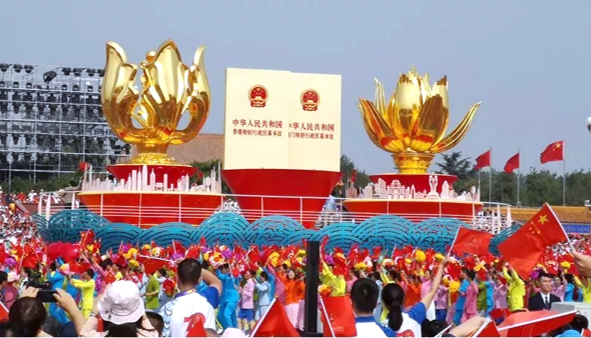
\includegraphics[width=\textwidth]{./resources/27.png}
    \end{columns}
\end{frame}

\begin{frame}{建党百年}
    \begin{columns}
        \column{0.4\textwidth}
        \setlength{\parindent}{2em}

        由北邮 318 名师生组成的\textcolor{Fore}{\textbf{庆祝中国共产党成立 100 周年大会}}广场合唱团、献词团、志愿者服务团,
        圆满完成庆祝大会演出及服务保障工作,把最优的精神面貌,最美的祝福赞歌,最亮的青年呼声汇聚成一份最真挚的青春献礼,向党和人民交上一份满意答卷。

        \column{0.6\textwidth}
        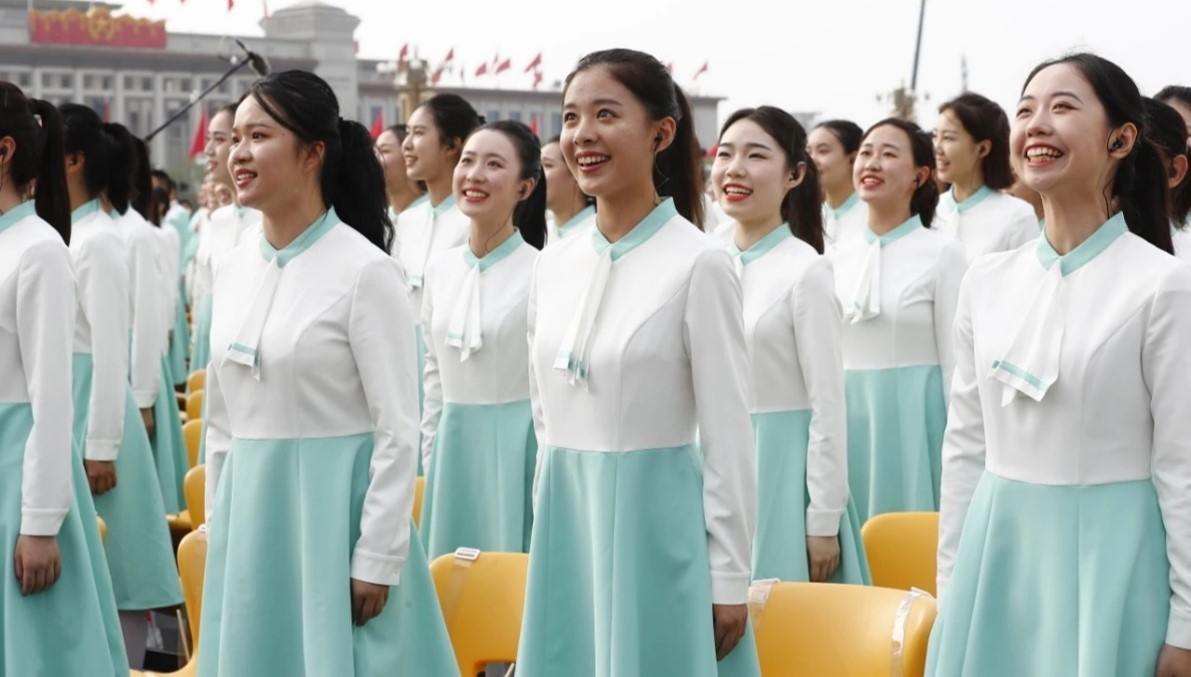
\includegraphics[width=\textwidth]{./resources/28.jpg}
    \end{columns}
\end{frame}

\begin{frame}{北京冬奥}
    \begin{columns}
        \column{0.35\textwidth}
        \setlength{\parindent}{2em}

        \textcolor{Fore}{\textbf{北京 2022 年冬奥会和冬残奥会}}期间,北京邮电大学作为\textcolor{Fore}{\textbf{主责高校}},
        与三所配合高校共同负责北京奥林匹克公园公共区的志愿服务工作。655 名志愿者用阳光、友好、青春的笑容,展现当代青年的责任与担当。

        \column{0.65\textwidth}
        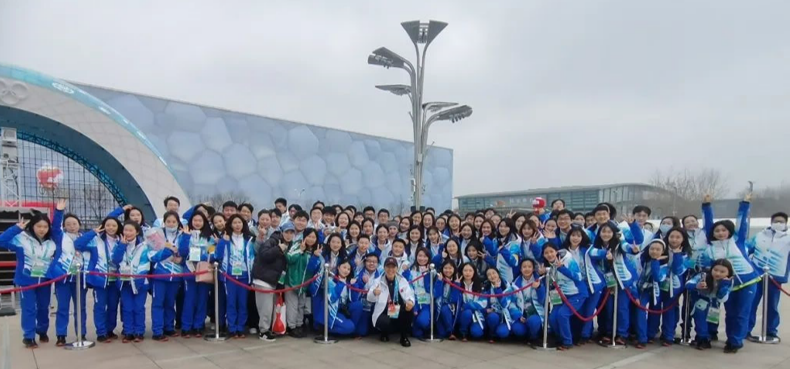
\includegraphics[width=\textwidth]{./resources/29.png}
    \end{columns}
\end{frame}

\section{录取情况}

\begin{frame}{目录}
    \begin{multicols}{2}
        \tableofcontents[currentsection]
    \end{multicols}
\end{frame}

\subsection*{江苏省 2022 年分专业(类)录取情况}

\begin{frame}{首选物理普通专业组}
    \begin{table}
        \small
        \centering
        \arrayrulecolor{Fore}
        \begin{tabular}{lcccc}
            \toprule
            \textcolor{Fore}{\textbf{大类/专业名称}}       & \textcolor{Fore}{\textbf{录取人数}} & \textcolor{Fore}{\textbf{最高分}} & \textcolor{Fore}{\textbf{最低分}} & \textcolor{Fore}{\textbf{平均分}} \\ \midrule
            通信工程(大类招生)                               & 11                              & 626                            & 623                            & 624                            \\
            电子信息类                                    & 6                               & 623                            & 622                            & 623                            \\
            计算机类                                     & 7                               & 630                            & 626                            & 628                            \\
            网络空间安全(大类招生)                             & 6                               & 625                            & 622                            & 623                            \\
            人工智能(大类招生)                               & 11                              & 624                            & 622                            & 622                            \\
            自动化类(智能机器人与智慧物流)                         & 5                               & 625                            & 621                            & 622                            \\
            大数据管理与应用                                 & 1                               & 622                            & 622                            & 622                            \\
            智能交互设计                                   & 1                               & 621                            & 621                            & 621                            \\
            \textcolor{Fore}{\textbf{总计(首选物理普通专业组)}} & \textcolor{Fore}{\textbf{48}}   & \textcolor{Fore}{\textbf{630}} & \textcolor{Fore}{\textbf{621}} & \textcolor{Fore}{\textbf{624}} \\ \midrule
        \end{tabular}
    \end{table}
\end{frame}

\begin{frame}{中外合作办学专业组}
    \begin{table}
        \centering
        \arrayrulecolor{Fore}
        \begin{tabular}{lcccc}
            \toprule
            \textcolor{Fore}{\textbf{大类/专业名称}}       & \textcolor{Fore}{\textbf{录取人数}} & \textcolor{Fore}{\textbf{最高分}} & \textcolor{Fore}{\textbf{最低分}} & \textcolor{Fore}{\textbf{平均分}} \\ \midrule
            电信工程及管理(中外合作办学)                          & 2                               & 610                            & 609                            & 610                            \\
            物联网工程(中外合作办学)                            & 2                               & 621                            & 609                            & 615                            \\
            \textcolor{Fore}{\textbf{总计(中外合作办学专业组)}} & \textcolor{Fore}{\textbf{4}}    & \textcolor{Fore}{\textbf{621}} & \textcolor{Fore}{\textbf{609}} & \textcolor{Fore}{\textbf{612}} \\ \midrule
        \end{tabular}
    \end{table}
\end{frame}

\section{相关问题}

\begin{frame}{目录}
    \begin{multicols}{2}
        \tableofcontents[currentsection]
    \end{multicols}
\end{frame}

\begin{frame}{转专业政策}
    为了充分调动学生学习的积极性和主动性,我校对于大部分专业实施转专业申请\textcolor{Fore}{\textbf{零门槛}}政策,让学生们有机会根据自己的兴趣、特长和爱好选择适合自己的专业,
    \textcolor{Fore}{\textbf{大一上学期结束}}和\textcolor{Fore}{\textbf{大一下学期结束时}},分别有一次申请转专业的机会,具体以教务处最新转专业政策为准。

    其中,高水平运动队、艺术类专业学生\textcolor{Fore}{\textbf{不得}}申请转专业,
    中外合作办学专业的学生\textcolor{Fore}{\textbf{不得}}申请转专业,
    其他非中外合作办学专业的学生\textcolor{Fore}{\textbf{不得}}申请转入中外合作办学专业。

    近几年我校转专业申请的学生中,\textcolor{Fore}{\textbf{总体成功率接近 70\%}}。
\end{frame}

\begin{frame}{保研政策}
    近几年来我校推荐免试研究生的比例一般在 \textcolor{Fore}{\textbf{23\% 左右}}(具体指标根据教育部每年相关规定确定),主要根据学生大学前三年的综合排名确定推免资格。

    同时,根据教育部文件精神,我校每年在优秀应届本科毕业生中,招收具有当年推荐免试资格的部分毕业生直接攻读博士研究生。
\end{frame}

\begin{frame}{学生奖励}
    \small
    \begin{itemize}
        \item \textcolor{Fore}{\textbf{国家奖学金}}
              每学年评选一次,每人每年 8000 元,二年级以上(含二年级)的品学兼优的在校本科生均可申请。
        \item \textcolor{Fore}{\textbf{国家励志奖学金}}
              每学年评选一次,每人每年 5000 元。
        \item \textcolor{Fore}{\textbf{学校奖学金}}
              一等奖学金每人 5000 元;二等奖学金每人 3000 元;三等奖学金每人 1000 元。
        \item \textcolor{Fore}{\textbf{社会赞助奖助学金}}
              目前近二十家企业在学校设立了奖助学金项目,每年奖助总金额 102.5 万元。
        \item \textcolor{Fore}{\textbf{其他荣誉奖项}}
              市级及校级三好学生、市级及校级优秀学生干部、优秀党员、优秀团干部、优秀团员、优秀毕业生、文体积极分子、学习进步奖、各类学科竞赛奖及文体活动奖等。
    \end{itemize}
\end{frame}

\begin{frame}{学生奖励}
    \begin{block}{2020—2021 学年}
        \begin{multicols}{3}
            \begin{center}
                国家奖学金

                \textcolor{Fore}{\textbf{\Large{1,016,000 元}}}\\[1em]
            \end{center}

            \begin{center}
                国家励志奖学金

                \textcolor{Fore}{\textbf{\Large{2,165,000 元}}}\\[1em]
            \end{center}

            \begin{center}
                学校奖学金

                \textcolor{Fore}{\textbf{\Large{7,943,000 元}}}\\[1em]
            \end{center}

            \begin{center}
                社会赞助奖学金

                \textcolor{Fore}{\textbf{\Large{1,000,000$^+$ 元}}}\\[1em]
            \end{center}

            \begin{center}
                其他荣誉奖项

                \textcolor{Fore}{\textbf{\Large{1,217,000 元}}}\\[1em]
            \end{center}
        \end{multicols}
    \end{block}

    我校每学年本科学生奖学金覆盖率\textcolor{Fore}{\textbf{近 60\%}}。
\end{frame}

\begin{frame}{助学体系}
    新生报到时,家庭经济特别困难的学生可以通过“绿色通道”缓交学费,先行入学并获得生活补助。

    入学后,来自低收入家庭的学生可申请\textcolor{Fore}{\textbf{国家助学贷款}}、\textcolor{Fore}{\textbf{国家助学金}}、
    \textcolor{Fore}{\textbf{临时困难补助}}、\textcolor{Fore}{\textbf{服兵役学生国家教育资助}}及\textcolor{Fore}{\textbf{勤工助学}}。

    家庭经济困难学生可申请办理国家助学贷款,每生每年最高不超过 12000 元,在校期间利息由国家承担。

    学校设立了教学科研助理、行政管理助理和学校公共服务等一系列校内勤工助学固定岗位和临时性岗位,工资标准按 \textcolor{Fore}{\textbf{20 元/小时}}发放。
\end{frame}

\begin{frame}{助学体系}
    \textcolor{Fore}{\textbf{临时困难补助}}是学校为帮助因突发事件导致经济困难的学生设立的一种临时性补助,
    学生在校期间遇突发事件或意外情况导致经济困难,可自愿提出申请,提交有关证明材料,学校视情况发放 1000—3000 元临时困难补助。

    学校通过分析每学期学生在校消费数据,对消费远低于全校平均水平的部分学生实施\textcolor{Fore}{\textbf{隐形资助}},发放餐补 960 元,直接发放至学生一卡通。
\end{frame}

\section*{总结}

\begin{frame}{传邮万里,国脉所系}
    \centering
    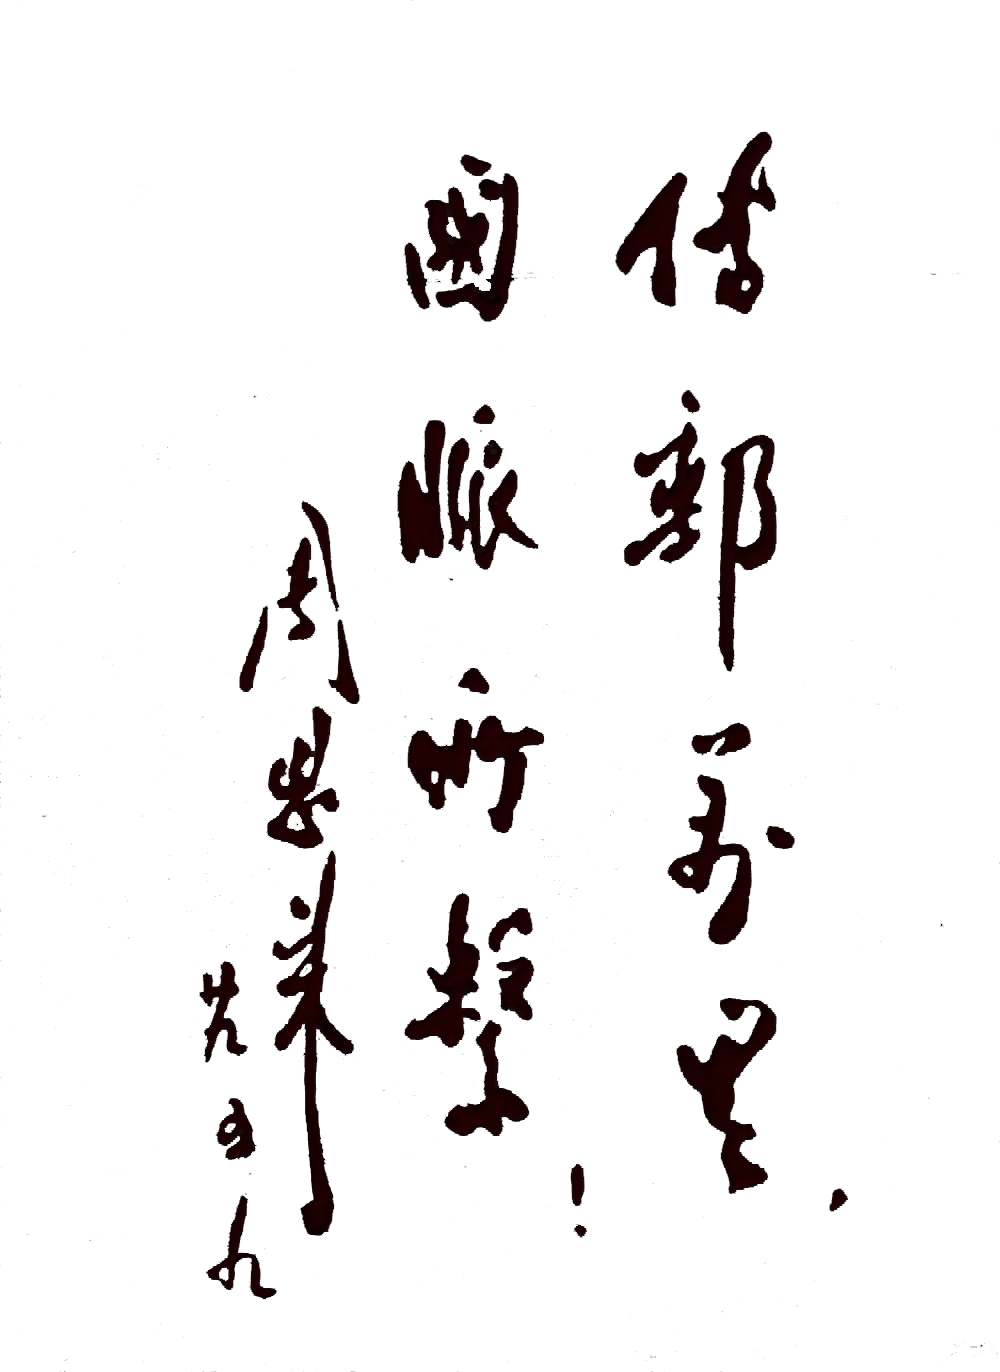
\includegraphics[width=0.3\textwidth]{./resources/30.png}
\end{frame}

\begin{frame}{欢迎报考信息黄埔}
    \small
    \begin{columns}
        \column{0.45\textwidth}
        \begin{itemize}
            \item \textcolor{Fore}{\textbf{北京邮电大学主页}}

                  \href{https://www.bupt.edu.cn}{https://www.bupt.edu.cn}

            \item \textcolor{Fore}{\textbf{北京邮电大学本科招生}}

                  \href{https://zsb.bupt.edu.cn}{https://zsb.bupt.edu.cn}

            \item \textcolor{Fore}{\textbf{电话}}

                  010-62282045, 010-62285045

                  010-62280945, 010-62289945

            \item \textcolor{Fore}{\textbf{招生办邮箱}}

                  \href{mailto://zsb@bupt.edu.cn}{zsb@bupt.edu.cn}
        \end{itemize}

        \column{0.6\textwidth}
        \begin{multicols}{3}
            \begin{center}
                \qrcode[hyperlink]{http://weixin.qq.com/r/gHS-p9HETYwyrZXE9yGS}\\[1em]

                \scriptsize
                北京邮电大学\\微信公众号
            \end{center}

            \begin{center}
                \qrcode[hyperlink]{http://weixin.qq.com/r/E3UZFnHEgU-_h2B1nyA3}\\[1em]

                \scriptsize
                北邮本科招生\\微信公众号
            \end{center}

            \begin{center}
                \qrcode[hyperlink]{https://qm.qq.com/cgi-bin/qm/qr?k=uqV2JgRErxR_U93VWdbLQCQ6pvgJY6cy&authKey=l9P17guN99DDaQbTghm6qGSlGyQFG6H+PY3pb8Fjbpu4RorvXL3epnXxZY1J9XOf&noverify=0}\\[1em]

                \scriptsize
                北邮 JYGZ\\宣讲 QQ 群
            \end{center}

        \end{multicols}

        \textcolor{Fore}{\textbf{幻灯片源代码}}

        \href{https://github.com/XIA-Jinyi/BuptToJygz2023}{https://github.com/XIA-Jinyi/BuptToJygz2023}
    \end{columns}
\end{frame}

\end{document}